% Q13/Q16 -- 4:1 MUX nMOS STICK diagram (simplified, colour-coded layers).
% poly = red (select lines), n-diffusion = green (data rows), metal = blue (output bus),
% contacts = black squares. A poly line crossing a diffusion row = a pass transistor gate.
\documentclass[border=10pt]{standalone}
\usepackage{tikz}
\begin{document}
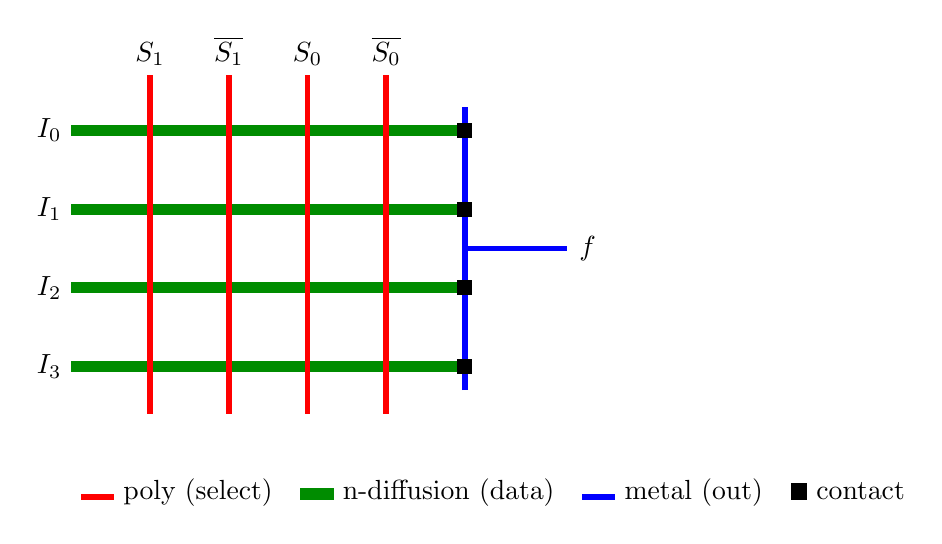
\begin{tikzpicture}[
  poly/.style={red, line width=2pt},
  ndiff/.style={green!55!black, line width=4pt},
  metal/.style={blue, line width=2pt},
  cont/.style={fill=black, draw=black, minimum size=5pt, inner sep=0pt}]
% data rows (n-diffusion)
\foreach \r/\lbl in {4/$I_0$,3/$I_1$,2/$I_2$,1/$I_3$}{
  \draw[ndiff] (1,\r) -- (6,\r);
  \node[left] at (1,\r) {\lbl};
}
% select lines (poly)
\foreach \c/\lbl in {2/$S_1$,3/$\overline{S_1}$,4/$S_0$,5/$\overline{S_0}$}{
  \draw[poly] (\c,0.4) -- (\c,4.7);
  \node[above] at (\c,4.7) {\lbl};
}
% output metal bus -> f
\draw[metal] (6,0.7) -- (6,4.3);
\draw[metal] (6,2.5) -- (7.3,2.5) node[right, black]{$f$};
% contacts where each diffusion row meets the output metal bus
\foreach \r in {1,2,3,4}{ \node[cont] at (6,\r) {}; }
% legend
\node[anchor=west, align=left] at (1,-0.6)
 {\textcolor{red}{$\rule{12pt}{2pt}$} poly (select)\quad
  \textcolor{green!55!black}{$\rule{12pt}{4pt}$} n-diffusion (data)\quad
  \textcolor{blue}{$\rule{12pt}{2pt}$} metal (out)\quad
  \rule{6pt}{6pt}~contact};
\end{tikzpicture}
\end{document}
